
\documentclass[xcolor=svgnames,final,smaller,a4]{beamer}
\usepackage{relsize}
\usepackage{luacode}
\usepackage{xcolor}
\usepackage{alltt}
\usepackage{wasysym}
\usepackage{hyperref}
\usepackage{newunicodechar}

\hypersetup{
  colorlinks   = true, %Colours links instead of ugly boxes
  urlcolor     = NavyBlue, %Colour for external hyperlinks
  linkcolor    = DarkGreen, %Colour of internal links
  citecolor   = DarkMagenta, %Colour of citations
  frenchlinks = true,
}
\begin{document}
 \begin{luacode*}
   local gitpip=io.popen("git log --no-color --format=oneline -1 --abbrev=16 --abbrev-commit -q | cut -d' ' -f1")
   gitid=gitpip:read()
   gitpip:close()
 \end{luacode*}
 \newcommand{\mygitid}{\luadirect{tex.print(gitid)}}


 \begin{frame}
   {compléments sur les architectures}

   \begin{center}
     
     
\includegraphics[width=0.1\textwidth]{cc-by-nc-sa} Basile \textsc{Starynkévitch} - mars 2023

     git {\texttt \mygitid}
   \end{center}
 \end{frame}


 \begin{frame}{architecture x86-64}

   \href{https://www.amd.com/system/files/TechDocs/24592.pdf}{\texttt{https://www.amd.com/system/files/TechDocs/24592.pdf}}

   \begin{center}
   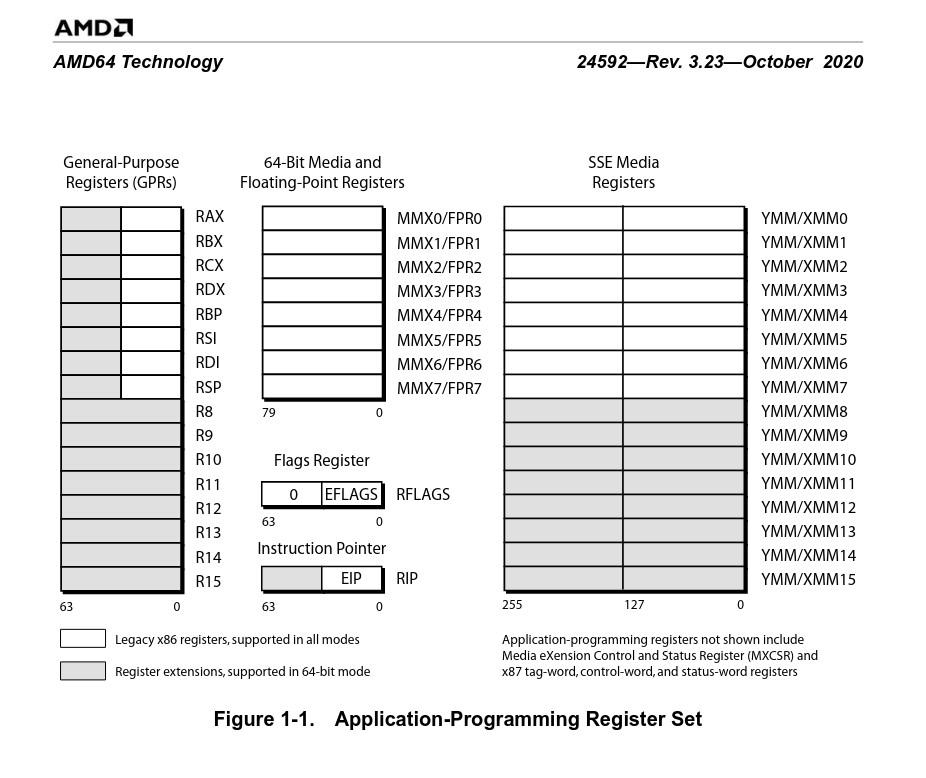
\includegraphics[width=0.85\textwidth]{amd64-registers.png}
   \end{center}
   
 \end{frame}


 \begin{frame}{modes d'exécution x86-64}

   \begin{center}
   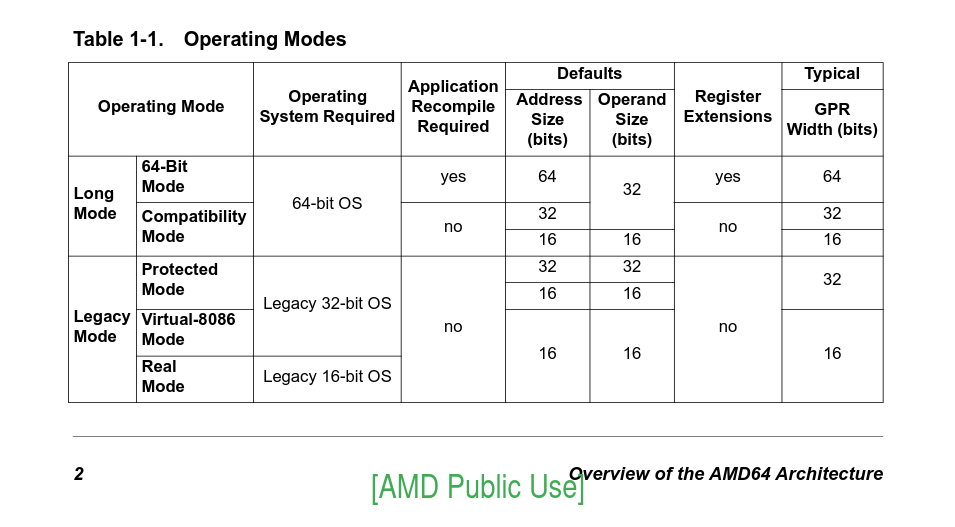
\includegraphics[width=0.85\textwidth]{amd64-opermodes.png}
   \end{center}
 \end{frame}


 \begin{frame}{appel en C de \texttt{fact(8)}

     \texttt{/*fichier f.c*/}
     
     \texttt{\textbf{extern} long fact(long);}

     \texttt{long calcfact8(void) \{}
     
     \texttt{\hspace{1cm}    long n = fact(8L);}

     \texttt{\hspace{1cm} \textbf{return} n;}

     \texttt{\} /* fin calcfact8 */}
     
 \end{frame}
\end{document}
#%%%%%%%%%%%%%%%%%%%%%%%%%%%%%%%%%%%%%%%%%%%%%%%%%%%%%%%%%%%%%%%
#% Local Variables: ;;
#% compile-command: "./build-archi2023.sh" ;;
#% End: ;;
#%%%%%%%%%%%%%%%%%%%%%%%%%%%%%%%%%%%%%%%%%%%%%%%%%%%%%%%%%%%%%%%
